\newgeometry{top=1cm, bottom=2cm}
\section{Matrizen}
\begin{figure}[h!]
    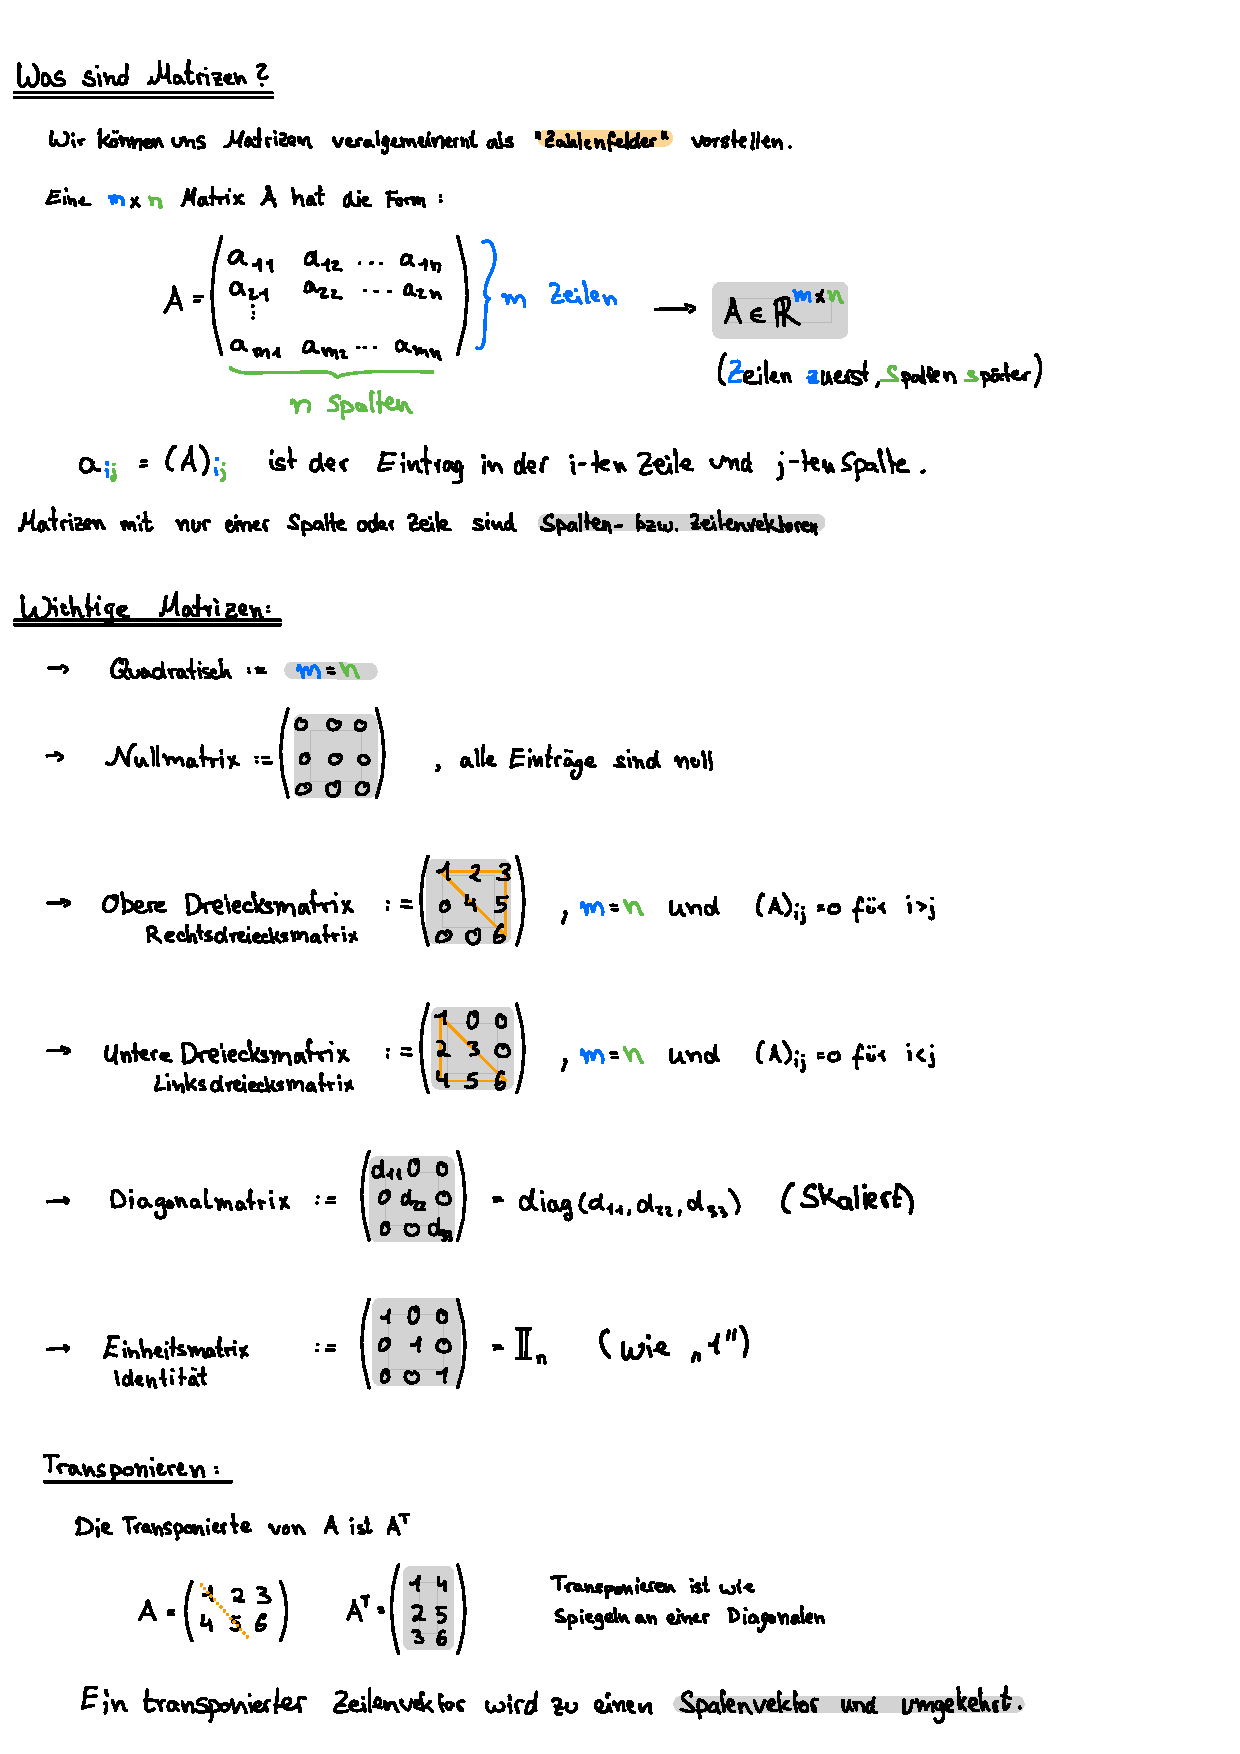
\includegraphics[page=1, scale=0.842]{pdf/02_Matrizen.pdf}
\end{figure}
\newpage
\includepdf[pages={2-}, 
            pagecommand={\thispagestyle{plain}}, 
            scale=0.95]{pdf/02_Matrizen.pdf}

\newgeometry{top=2.5cm, bottom=2cm}

\subsection{Beispielaufgaben} 

\vspace{1cm}

\subsubsection{} %Übung 06
Was ist
\begin{equation*}
    \begin{pmatrix}
    0 & 0 & 1 & 0
    \end{pmatrix}
    \begin{pmatrix}
    -1 & 1 & -1 & 2 \\
    0 & 2 & 0 & -1 \\
    -3 & 2 & -3 & 1 \\
    2 & 1 & 2 & 3 \\
    \end{pmatrix}
    \begin{pmatrix}
    -1 & 1 & -1 & 2 \\
    0 & 2 & 0 & -1 \\
    -3 & 2 & -3 & 1 \\
    2 & 1 & 2 & 3 \\
    \end{pmatrix}
    \begin{pmatrix}
    0\\
    1\\
    0\\
    0\\
    \end{pmatrix}?
\end{equation*}

\vspace{1\baselineskip}

\begin{solution}    

    \vspace{1\baselineskip}

    \leftskip=2em

    Wir können den komplexen Ausdruck etwas vereinfachen um die Rechnung zu erleichtern.

    \begin{equation*}    
        \begin{pmatrix}
        0 & 0 & 1 & 0
        \end{pmatrix}
        \begin{pmatrix}
        -1 & 1 & -1 & 2 \\
        0 & 2 & 0 & -1 \\
        -3 & 2 & -3 & 1 \\
        2 & 1 & 2 & 3 \\
        \end{pmatrix}
        \underbrace{
        \begin{pmatrix}
        -1 & 1 & -1 & 2 \\
        0 & 2 & 0 & -1 \\
        -3 & 2 & -3 & 1 \\
        2 & 1 & 2 & 3 \\
        \end{pmatrix}
        \begin{pmatrix}
        0\\
        1\\
        0\\
        0\\
        \end{pmatrix}}_{\text{Extrahiert die 2. Spalte der Matrix}}
    \end{equation*}

    \vspace{1\baselineskip}

    \begin{equation*}    
        \begin{pmatrix}
        0 & 0 & 1 & 0
        \end{pmatrix}
        \underbrace{
        \begin{pmatrix}
        -1 & 1 & -1 & 2 \\
        0 & 2 & 0 & -1 \\
        -3 & 2 & -3 & 1 \\
        2 & 1 & 2 & 3 \\
        \end{pmatrix}
        \begin{pmatrix}
            1 \\
            2 \\
            2 \\ 
            1 \\
        \end{pmatrix}}_{\begin{pmatrix} x_1 \\ x_2 \\ x_3 \\ x_4 \end{pmatrix}}
    \end{equation*}

    \vspace{1\baselineskip}

    \begin{equation*}
        \begin{pmatrix}
        0 & 0 & 1 & 0
        \end{pmatrix}
        \begin{pmatrix}
            x_1 \\
            x_2 \\
            x_3 \\
            x_4 
        \end{pmatrix}
        = x_3
    \end{equation*}

    Wir müssen also nur \( x_3 \) berechnen was durch das Produkt 
    
    \begin{equation*}
        \begin{pmatrix} -3 & 2 & -3 & 1 \end{pmatrix} \begin{pmatrix} 1 \\ 2 \\ 2 \\ 1 \end{pmatrix} 
    \end{equation*}

    gegeben ist. Das Resultat ist dann \( -4 \).  

\end{solution}

\newpage

\subsubsection{} %Adi PVK Tag 1
Für \( a \in \mathbb{R} \)  sei die Matrix

\begin{equation*}
    A = \begin{pmatrix}
    1 & 0 & 0 & 2 \\
    0 & 1 & 0 & 0 \\
    -1 & 0 & 1 & 0 \\
    a & 1 & 0 & 1 \\
    \end{pmatrix}
\end{equation*}

gegeben. Für welche Werte von \( a \) ist die Matrix \( A \) singulär bzw. regulär? Bestimmen Sie für \( a = 0 \) die Inverse von \( A \). 

\vspace{1\baselineskip}

\begin{solution}    

    \vspace{1\baselineskip}

    \leftskip=2em

    Singulär: wenn Zeilen/ Spalten linear abhängig sind. 

    Regulär: wenn Zeilen/ Spalten linear unabhängig sind.
    
    \vspace{1\baselineskip}

    Für \( a = 0.5 \)

    \begin{equation*}
        \begin{gmatrix}[p]
            1 & 0 & 0 & 2 \\
            0 & 1 & 0 & 0 \\
            -1 & 0 & 1 & 0 \\
            0.5 & 1 & 0 & 1 
                \rowops
                    \add[-1]{1}{3}
        \end{gmatrix} \rightarrow \quad   
        \begin{gmatrix}[p]
            1 & 0 & 0 & 2 \\
            0 & 1 & 0 & 0 \\
            -1 & 0 & 1 & 0 \\
            0.5 & 0 & 0 & 1
        \end{gmatrix} 
    \end{equation*}

    In diesem Fall sind die Zeilen I und IV linear abhängig. D.h. die Matrix ist singulär (nicht invertierbar).

    \vspace{1\baselineskip}

    Für \( a = 0 \) wenden wir den Gauss-Jordan Algorithmus an. 
    
    \begin{equation*}
        \begin{gmatrix}[L]
            1 & 0 & 0 & 2 \\
            0 & 1 & 0 & 0 \\
            -1 & 0 & 1 & 0 \\
            0 & 1 & 0 & 1 
        \end{gmatrix} \hspace{-0.75em}
        \begin{gmatrix}[R]
            1 & 0 & 0 & 0 \\
            0 & 1 & 0 & 0 \\
            0 & 0 & 1 & 0 \\
            0 & 0 & 0 & 1
                \rowops
                    \add[1]{0}{2}
                    \add[-1]{1}{3}
        \end{gmatrix} \rightarrow \quad
        \begin{gmatrix}[L]
            1 & 0 & 0 & 2 \\
            0 & 1 & 0 & 0 \\
            0 & 0 & 1 & 2 \\
            0 & 0 & 0 & 1
        \end{gmatrix} \hspace{-0.75em}
        \begin{gmatrix}[R]
            1 & 0 & 0 & 0 \\
            0 & 1 & 0 & 0 \\
            1 & 0 & 1 & 0 \\
            0 & -1 & 0 & 1
                \rowops
                    \add[-2]{3}{2}
                    \add[-2]{3}{0}
        \end{gmatrix}
    \end{equation*}

    \vspace{1\baselineskip}

    \begin{equation*}
        \begin{gmatrix}[L]
            1 & 0 & 0 & 0 \\
            0 & 1 & 0 & 0 \\
            0 & 0 & 1 & 0 \\
            0 & 0 & 0 & 1
        \end{gmatrix} \hspace{-0.75em}
        \underbrace{
        \begin{gmatrix}[R]
            1 & 2 & 0 & -2 \\
            0 & 1 & 0 & 0 \\
            1 & 2 & 1 & -2 \\
            0 & -1 & 0 & 1
            \end{gmatrix}}_{A^{-1}}
    \end{equation*}

\end{solution}

\newpage

\subsubsection{} %Zardini S.27
Bestimmen Sie die LR-Zerlegung der Matrix \( A \), so dass \( LR = PA \)

\begin{equation*}
    A = \begin{pmatrix}
    0 & 1 & -3 \\
    -3 & 7 & 6 \\
    -3 & -2 & -2 \\
    \end{pmatrix}.
\end{equation*}

\vspace{1\baselineskip}

\begin{solution}    

    \vspace{1\baselineskip}

    \leftskip=2em

    Wir wenden dafür das Rezept an und erhalten
    
    \begin{equation*}
        \begin{aligned}
            & \begin{gmatrix}[L]
                1 & 0 & 0 \\
                0 & 1 & 0 \\
                0 & 0 & 1
            \end{gmatrix} \hspace{-0.75em}
            \begin{gmatrix}[R]
                0 & 1 & -3 \\
                -3 & 7 & 6 \\
                -3 & -2 & -2
                    \rowops
                        \swap{0}{1}
            \end{gmatrix} \; \; \, \rightarrow \quad
            \begin{gmatrix}[L]
                0 & 1 & 0 \\
                1 & 0 & 0 \\
                0 & 0 & 1
            \end{gmatrix} \hspace{-0.75em}
            \begin{gmatrix}[R]
                -3 & 7 & 6 \\
                0 & 1 & -3 \\
                -3 & -2 & -2
                    \rowops
                        \add[-1]{0}{2}
            \end{gmatrix}  \\[1em]
            & \begin{gmatrix}[L]
                0 & 1 & 0 \\
                1 & 0 & 0 \\
                0 & 0 & 1
            \end{gmatrix} \hspace{-0.75em}
            \begin{gmatrix}[R]
                -3 & 7 & 6 \\
                0 & 1 & -3 \\
                \textcolor{red}{1} & -9 & -8
                    \rowops
                        \add[9]{1}{2}
            \end{gmatrix} \rightarrow \quad
            \begin{gmatrix}[L]
                0 & 1 & 0 \\
                1 & 0 & 0 \\
                0 & 0 & 1
            \end{gmatrix} \hspace{-0.75em}
            \begin{gmatrix}[R]
                -3 & 7 & 6 \\
                0 & 1 & -3 \\
                \textcolor{red}{1} & \textcolor{red}{-9} & -35
            \end{gmatrix}
        \end{aligned}
    \end{equation*}

    wobei die roten Einträge die Einträge der Matrix \( L \) sind. \( L,\ R \) und \( P \) sind dann gegeben durch
    \begin{equation*}
        L = \begin{pmatrix}
        1 & 0 & 0 \\
        0 & 1 & 0 \\
        1 & -9 & 1
        \end{pmatrix}, \quad
        R = \begin{pmatrix}
        -3 & 7 & 6 \\
        0 & 1 & -3 \\
        0 & 0 & -35
        \end{pmatrix}, \quad
        P = \begin{pmatrix}
        0 & 1 & 0 \\
        1 & 0 & 0 \\
        0 & 0 & 1
        \end{pmatrix}.
    \end{equation*}

\end{solution}